\chapter{Example graph}
\label{sec:example-graph}

\autoref{fig:example-graph-without-updates} shows a snapshot of an example graph.

\autoref{fig:example-graph-with-updates} shows an example graph with update operations.
Insertions are denoted with a green asterisk~
\includegraphics[scale=0.25]{patterns/insert}.
Deletions of a single element are denoted with a red cross~
\includegraphics[scale=0.25]{patterns/delete-single},
while recursive deletions are denoted with a purple cross~
\includegraphics[scale=0.25]{patterns/delete-recursively}.

\begin{figure}[ht]
    \centering
    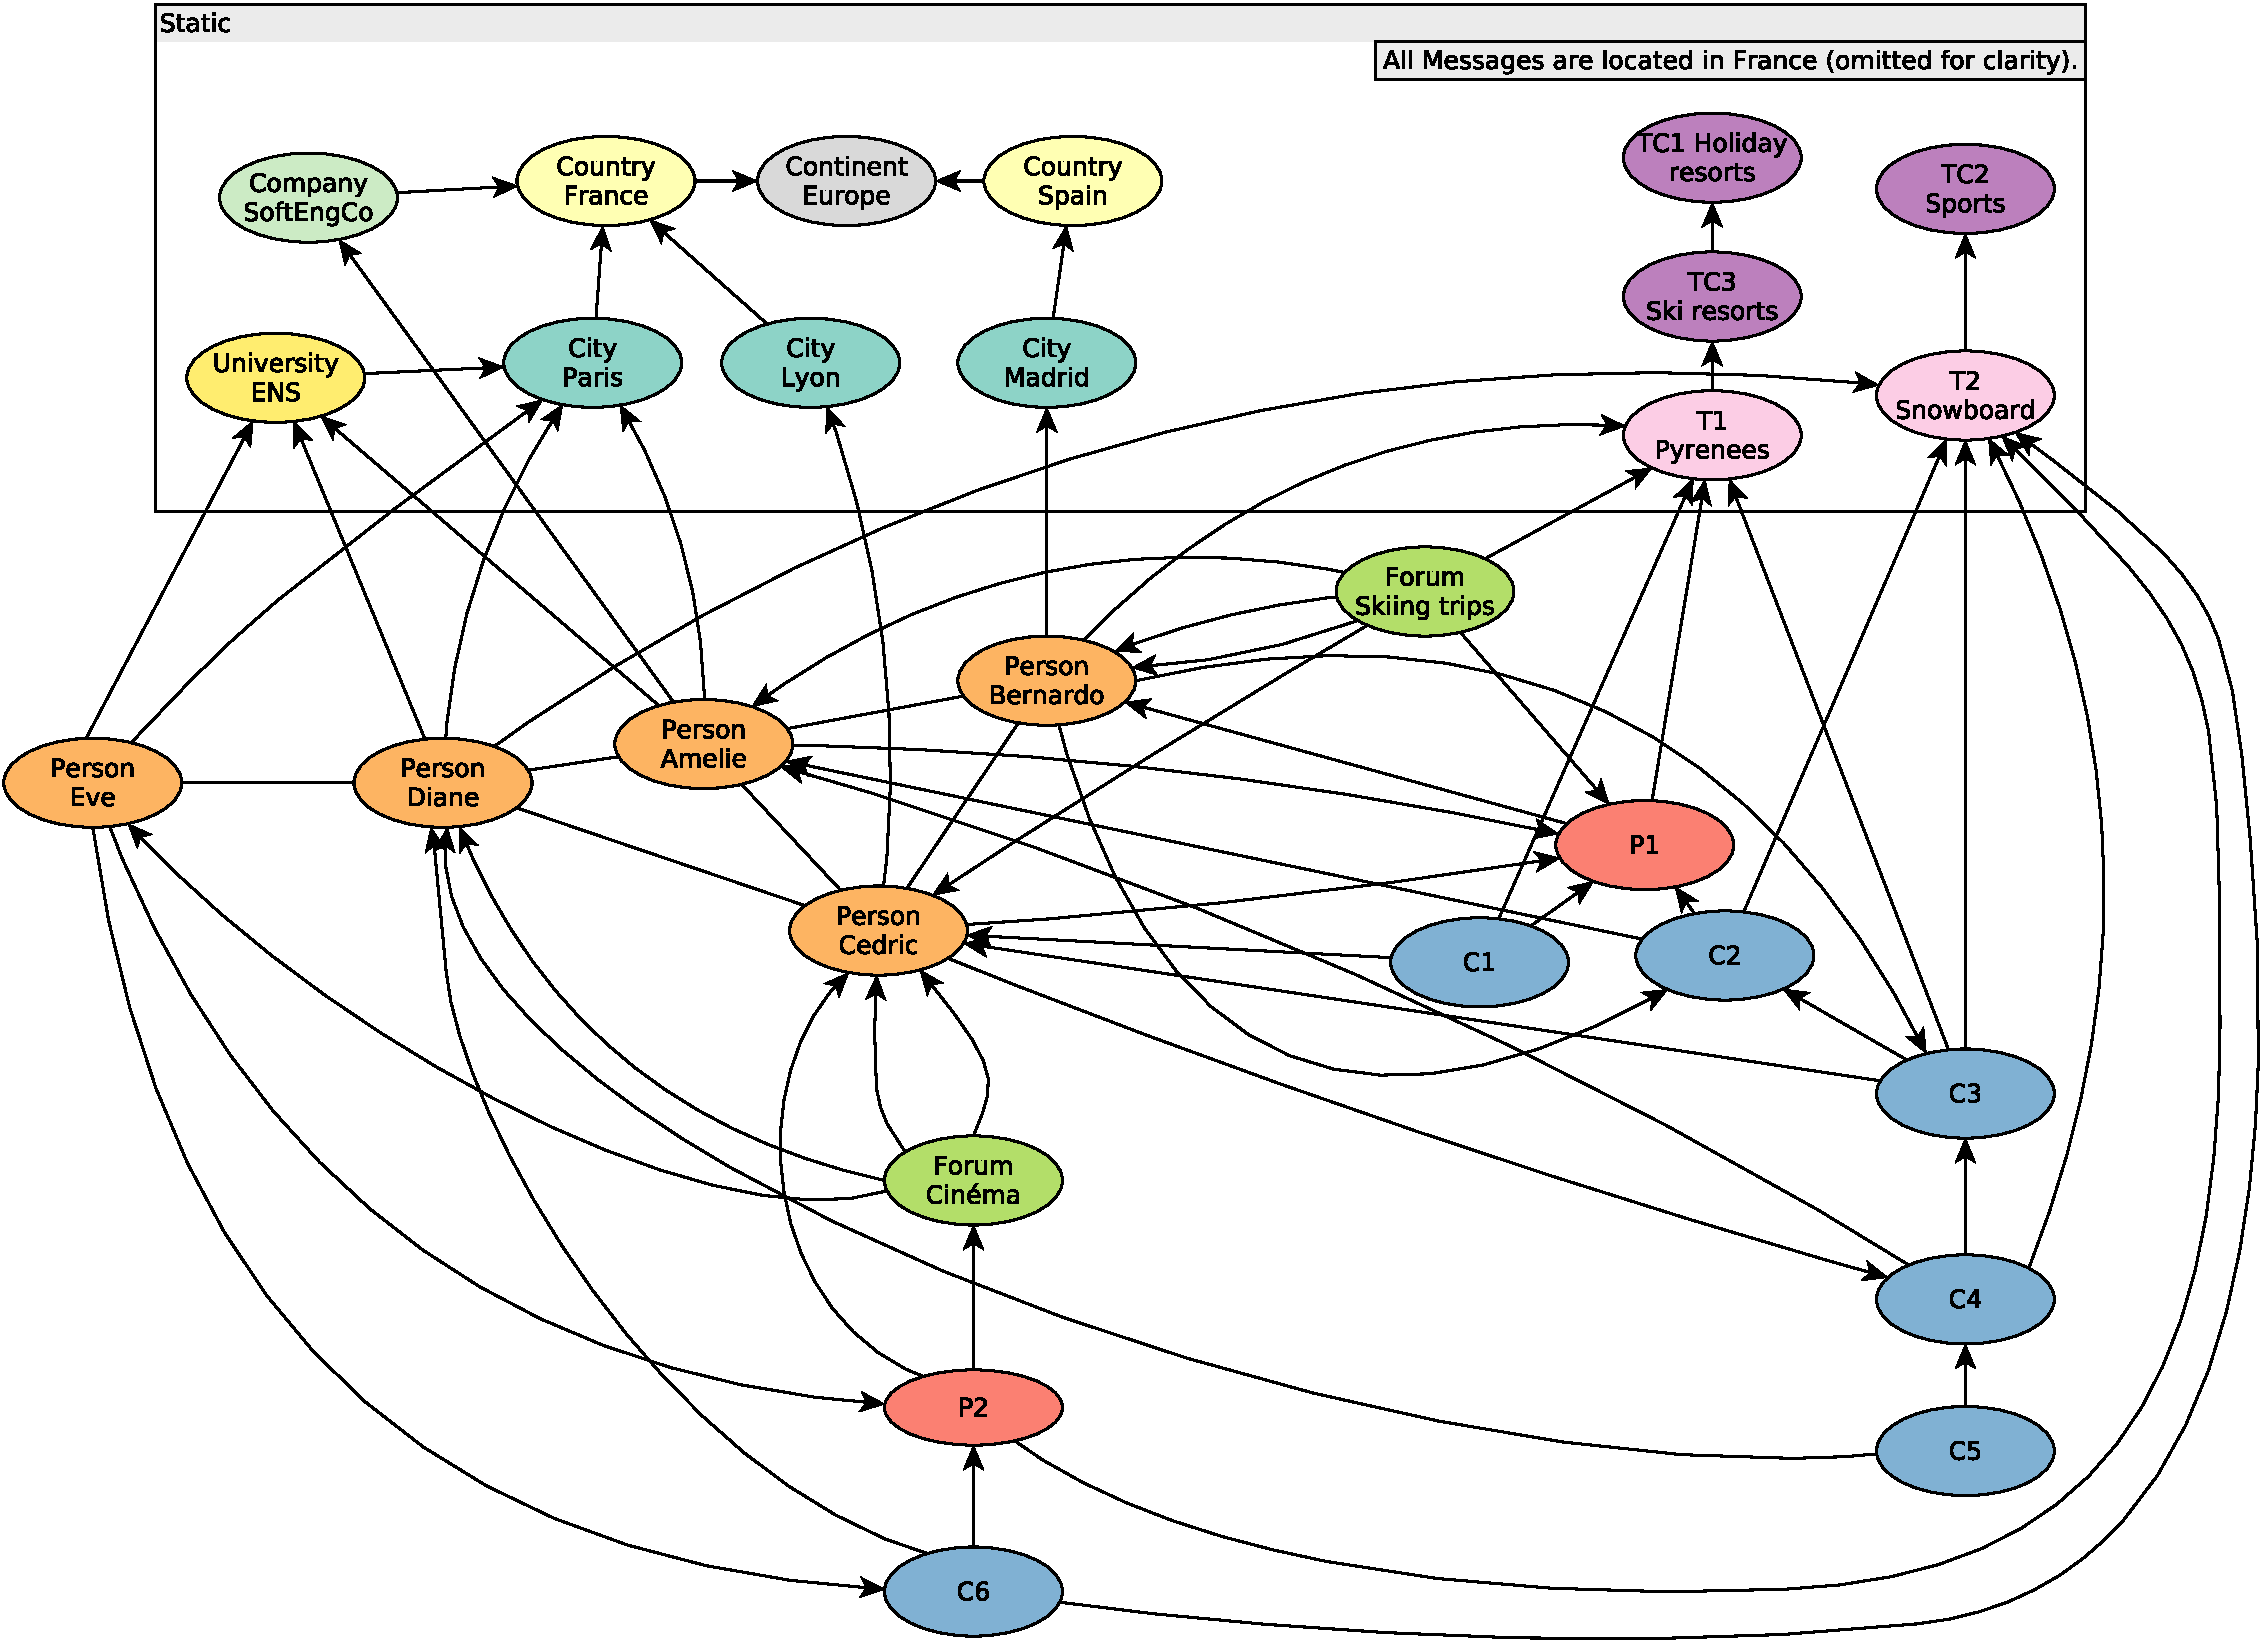
\includegraphics[scale=\yedscale]{figures/example-graph-without-updates}
    \caption{Example graph snapshot (without update operations).}
    \label{fig:example-graph-without-updates}
\end{figure}

\begin{figure}[ht]
    \centering
    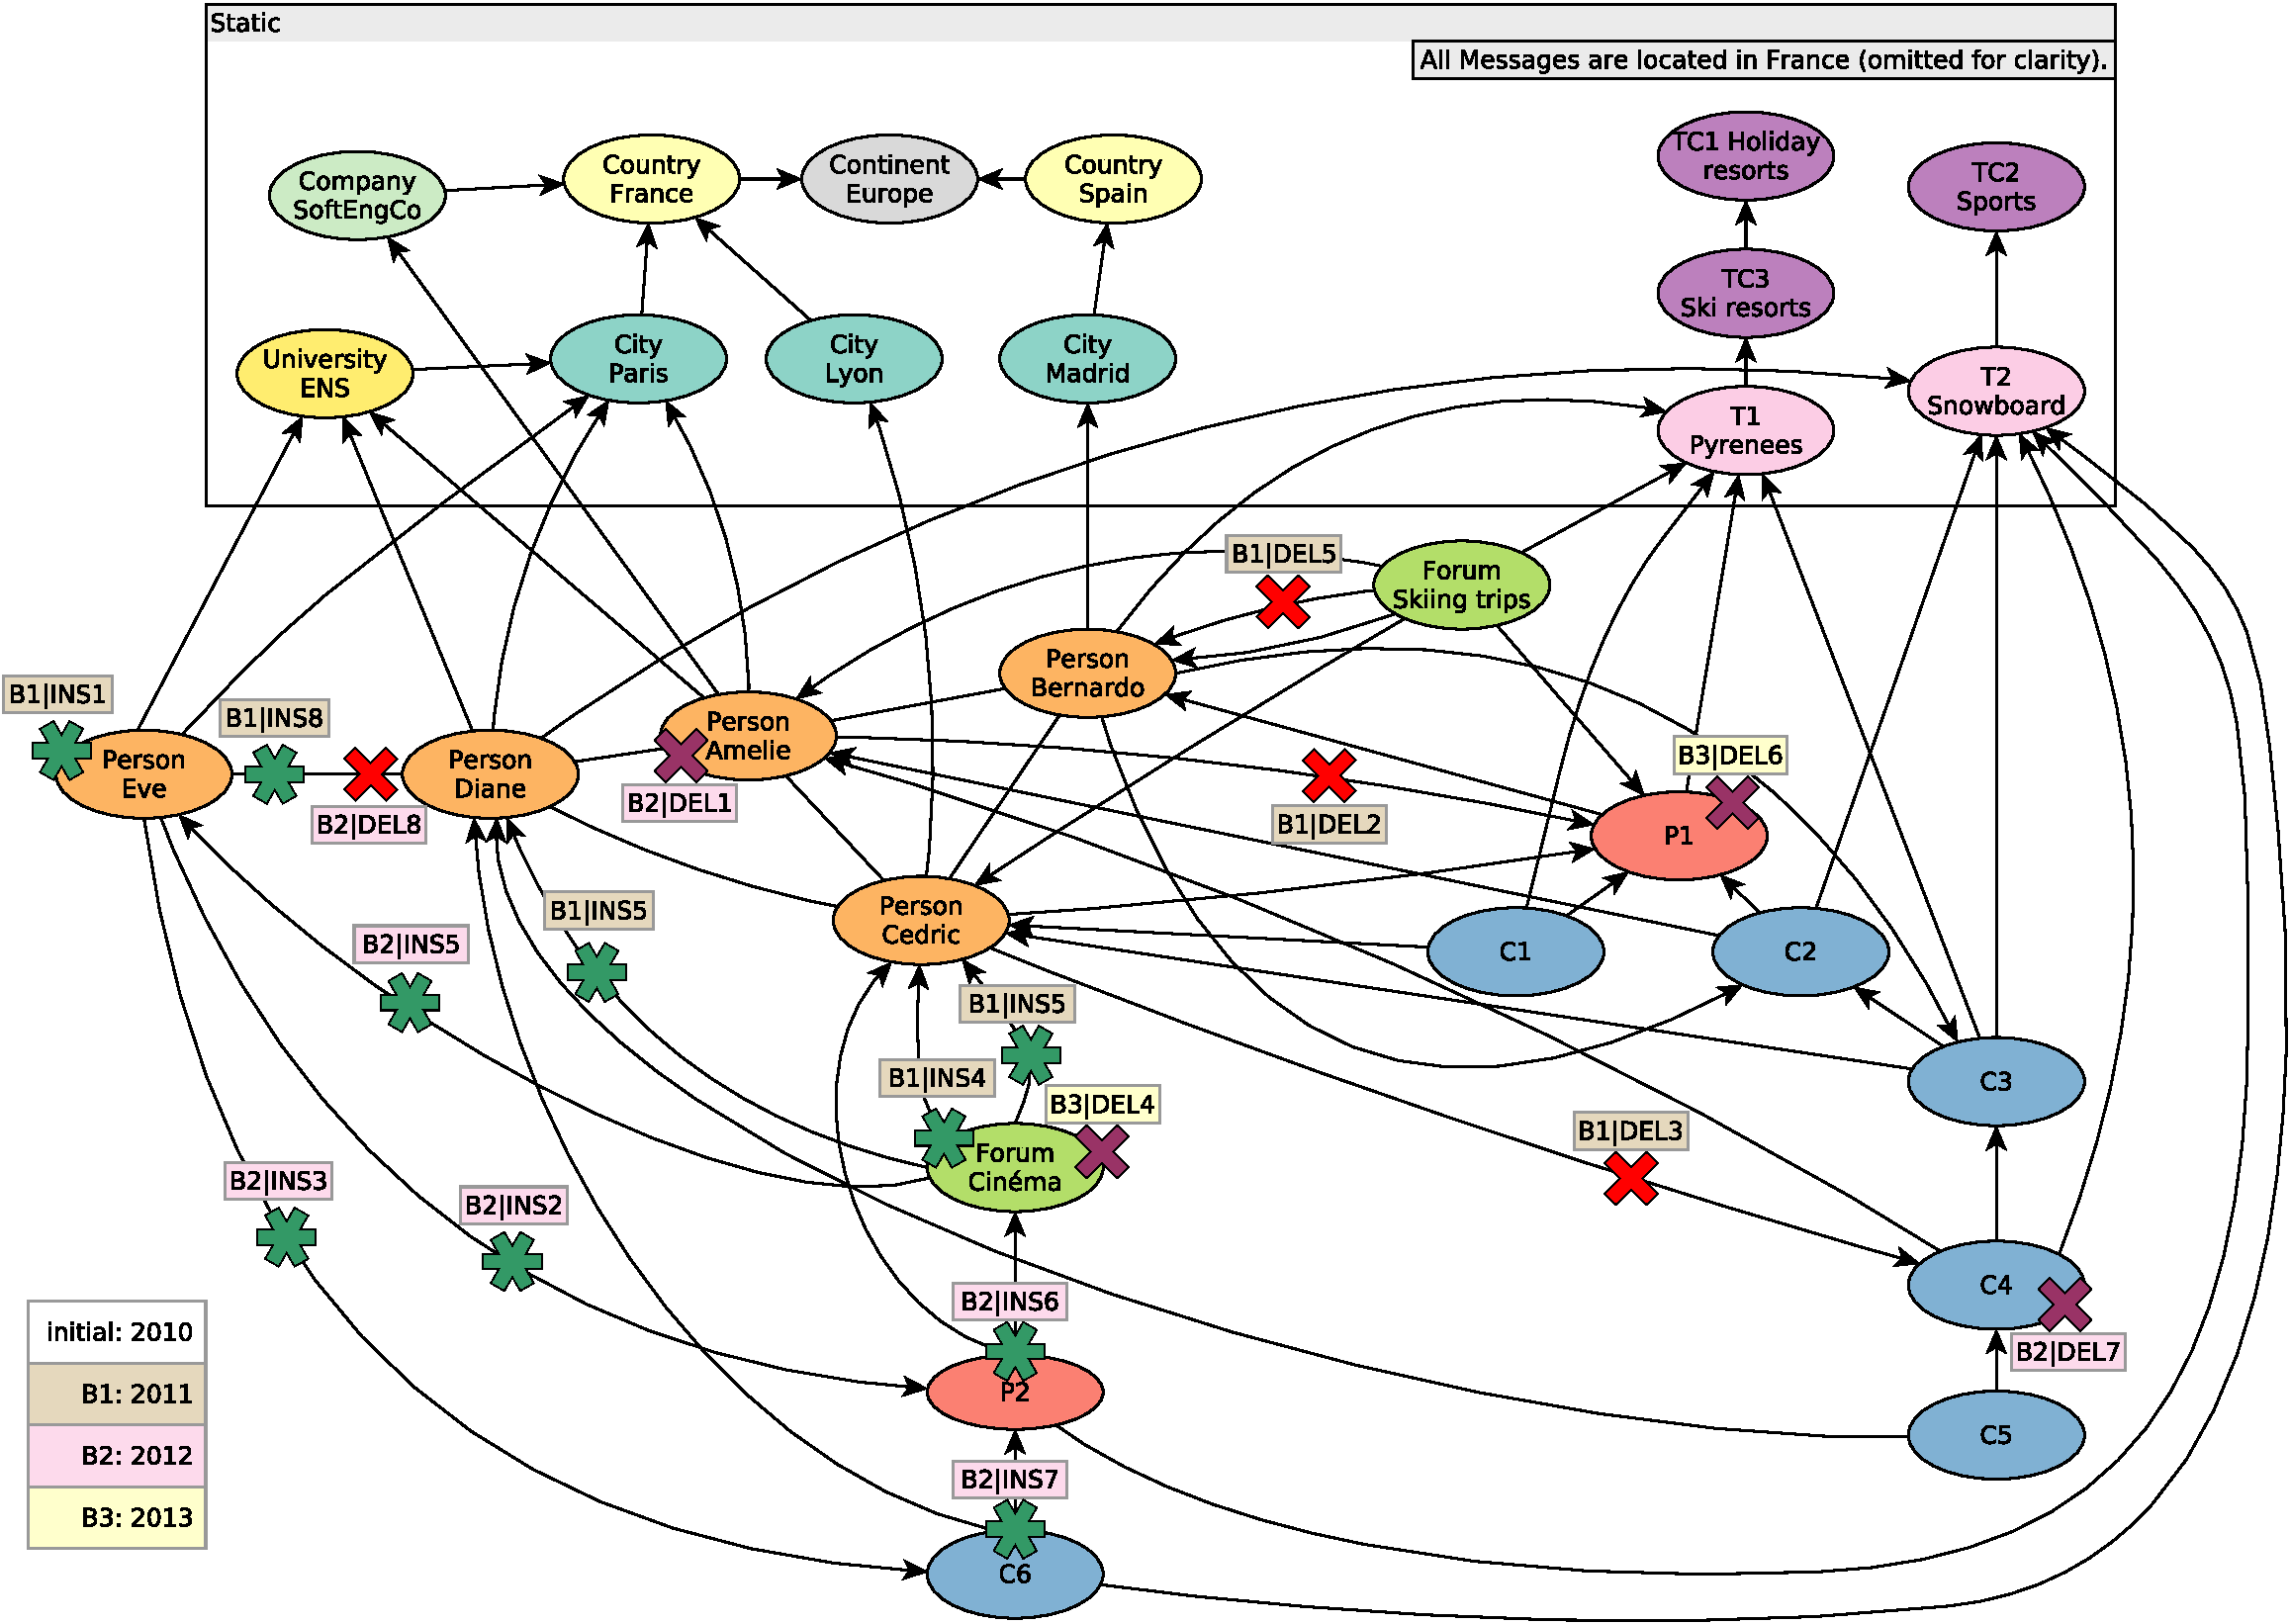
\includegraphics[scale=\yedscale]{figures/example-graph-with-updates}
    \caption{Example graph with update operations.}
    \label{fig:example-graph-with-updates}
\end{figure}
